\chapter{Technology and Operations}\label{ch:technology-and-operations}

\begin{importantbox}
Let me share something I learned the hard way: in Nigeria, technology isn't just about having the latest tools --- it's about having the right tools that work reliably in our unique environment. When I started Firmbird, I made the classic mistake of trying to replicate a Silicon Valley tech stack. Three power outages later, I learned that Nigerian tech operations require a different approach.
\end{importantbox}

\section{The Nigerian Tech Reality}\label{sec:nigerian-tech-reality}

``But Dele,'' a founder once told me, ``surely we just need to set up our usual systems here?'' I smiled, remembering my own journey. ``Let me show you something,'' I replied, ``See those buildings? Each one has adapted their tech to work with, not against, local realities.''

Let's start with what I call the ``Power-Internet-Backup'' (PIB) triangle --- the foundation of any successful tech operation in Nigeria:

\begin{figure}[h]
    \centering
    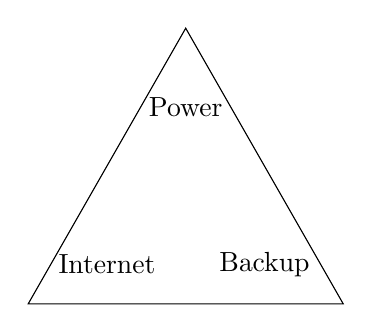
\begin{tikzpicture}
        % PIB Triangle visualization
        \draw (0,0) -- (4,0) -- (2,3.5) -- cycle;
        \node at (2,2.5) {Power};
        \node at (1,0.5) {Internet};
        \node at (3,0.5) {Backup};
    \end{tikzpicture}
    \caption{The PIB Triangle}
    \label{fig:pib-triangle}
\end{figure}

\section{Essential Infrastructure Setup}\label{sec:essential-infrastructure}

\subsection{Power Management}\label{subsec:power-management}
\begin{tcolorbox}[colback=white,colframe=primarydark,title=\textbf{Power Setup Essentials}]
\begin{itemize}
    \item \textbf{Primary UPS System}
    \begin{itemize}
        \item Minimum 2-hour backup for critical systems
        \item Automatic voltage regulation
        \item Equipment-grade surge protection
    \end{itemize}

    \item \textbf{Generator Strategy}
    \begin{itemize}
        \item Inverter-type generator for sensitive equipment
        \item Fuel monitoring system
        \item Regular maintenance schedule
    \end{itemize}

    \item \textbf{Power Optimization}
    \begin{itemize}
        \item Energy-efficient equipment selection
        \item Load balancing setup
        \item Power consumption monitoring
    \end{itemize}
\end{itemize}
\end{tcolorbox}

\subsection{Internet Redundancy}\label{subsec:internet-redundancy}
I learned this lesson during a crucial client presentation: never rely on a single internet connection. Here's my tried-and-tested approach:

\begin{center}
\begin{tabularx}{\textwidth}{>{\raggedright\arraybackslash}X >{\centering\arraybackslash}X >{\raggedright\arraybackslash}X}
    \toprule
    \textbf{Connection Type} & \textbf{Provider} & \textbf{Purpose} \\
    \midrule
    Primary Fiber & MTN/Airtel & Main operations \\
    4G Backup & Different provider & Failover connection \\
    Mobile Hotspot & Third provider & Emergency backup \\
    \bottomrule
\end{tabularx}
\end{center}

\section{Core Systems Selection}\label{sec:core-systems}

Remember what I call the ``Nigerian Tech Paradox'': the best system isn't always the most advanced --- it's the most adaptable. Here's my framework for system selection:

\begin{tcolorbox}[colback=white,colframe=primarydark,title=\textbf{Essential Systems Framework}]
\begin{enumerate}
    \item \textbf{Communication Systems}
    \begin{itemize}
        \item Business email (GSuite/Microsoft 365)
        \item WhatsApp Business account
        \item Local business phone number
        \item Video conferencing solution (Google Meet, cheaper)
    \end{itemize}

    \item \textbf{Operations Management}
    \begin{itemize}
        \item Cloud-based accounting software
        \item Basic CRM system
        \item Document management solution
        \item Team collaboration tools
    \end{itemize}

    \item \textbf{Payment Processing}
    \begin{itemize}
        \item Local payment gateway (Paystack/Flutterwave)
        \item International payment solution (Stripe)
        \item Mobile money integration
        \item Bank transfer system
    \end{itemize}
\end{enumerate}
\end{tcolorbox}

\section{Security and Data Protection}\label{sec:security-data}

When a US-based entrepreneur asked me about security, I shared what I call the ``Market Stall Principle'' --- just as Nigerian market traders have multilayered security for their shops, your tech security needs multiple layers:

\begin{tcolorbox}[colback=white,colframe=primarydark,title=\textbf{Security Framework}]
\begin{itemize}
    \item \textbf{Basic Security}
    \begin{itemize}
        \item Password manager deployment
        \item Two-factor authentication
        \item Regular backup system
        \item Basic firewall setup
    \end{itemize}

    \item \textbf{Data Protection}
    \begin{itemize}
        \item Local data privacy compliance
        \item Secure file sharing protocols
        \item Customer data protection
        \item Access control systems
    \end{itemize}
\end{itemize}
\end{tcolorbox}

\section{Operations Management}\label{sec:operations-management}

Here's what I call the ``Daily Dance'' --- the rhythm of successful Nigerian operations:

\begin{center}
\begin{tabularx}{\textwidth}{>{\raggedright\arraybackslash}X >{\raggedright\arraybackslash}X}
    \toprule
    \textbf{Time} & \textbf{Operations Check} \\
    \midrule
    Morning & Power systems verification \\
    Mid-morning & Communication systems check \\
    Afternoon & Payment systems monitoring \\
    Evening & Data backup confirmation \\
    \bottomrule
\end{tabularx}
\end{center}

\section{Quality Control Systems}\label{sec:quality-control}

Quality control in Nigeria requires what I call the ``Triple-A Approach'':

\begin{figure}[h]
    \centering
    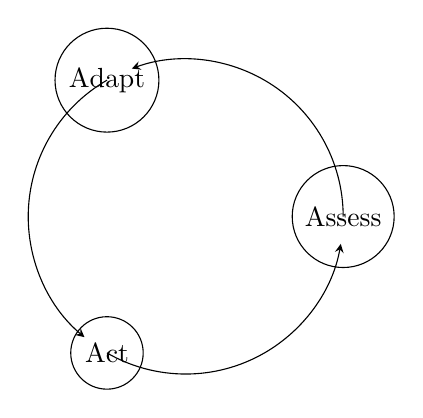
\begin{tikzpicture}
        \foreach \angle/\label in {
            0/Assess,
            120/Adapt,
            240/Act
        } {
            \node[draw, circle] at (\angle:2) {\label};
            \draw[-stealth] (\angle:2) arc (\angle:\angle+110:2);
        }
    \end{tikzpicture}
    \caption{Triple-A Quality Control}
    \label{fig:quality-control}
\end{figure}

\section{Implementation Timeline}\label{sec:implementation-timeline}

Let me share what I call the ``Four-Week Foundation'' --- a proven timeline for setting up your tech operations:

\begin{tcolorbox}[colback=white,colframe=primarydark,title=\textbf{Implementation Schedule}]
\begin{itemize}
    \item \textbf{Week 1: Basic Infrastructure}
    \begin{itemize}
        \item Power systems setup
        \item Internet connectivity
        \item Basic communication tools
    \end{itemize}

    \item \textbf{Week 2: Core Systems}
    \begin{itemize}
        \item Software deployment
        \item Payment integration
        \item Security implementation
    \end{itemize}

    \item \textbf{Week 3: Team Setup}
    \begin{itemize}
        \item Staff training
        \item Process documentation
        \item Systems testing
    \end{itemize}

    \item \textbf{Week 4: Optimization}
    \begin{itemize}
        \item Performance testing
        \item Backup verification
        \item Fine-tuning operations
    \end{itemize}
\end{itemize}
\end{tcolorbox}

\begin{workshopbox}
\textbf{Technology Setup Workshop}

1. Infrastructure Assessment
\begin{itemize}
    \item Power requirements: \_\_\_\_\_\_\_\_\_
    \item Internet needs: \_\_\_\_\_\_\_\_\_
    \item Backup systems: \_\_\_\_\_\_\_\_\_
\end{itemize}

2. Systems Planning
\begin{itemize}
    \item Core software needs: \_\_\_\_\_\_\_\_\_
    \item Integration requirements: \_\_\_\_\_\_\_\_\_
    \item Security priorities: \_\_\_\_\_\_\_\_\_
\end{itemize}

3. Operations Framework
\begin{itemize}
    \item Daily procedures: \_\_\_\_\_\_\_\_\_
    \item Quality controls: \_\_\_\_\_\_\_\_\_
    \item Emergency protocols: \_\_\_\_\_\_\_\_\_
\end{itemize}
\end{workshopbox}

\begin{communitybox}
Access additional resources on the Africa Growth Circle:
\begin{itemize}
    \item Vendor recommendations
    \item Setup guides and templates
    \item Expert tech support network
    \item Best practices documentation
\end{itemize}
Visit circle.counseal.com for technology support.
\end{communitybox}

\begin{importantbox}
Remember, successful tech operations in Nigeria isn't about having the most advanced systems --- it's about having the most reliable ones. In Chapter 9, we'll explore how to scale these systems as your business grows.
\end{importantbox}